\documentclass[20pt]{sigchi}


% Use this section to set the ACM copyright statement (e.g. for
% preprints).  Consult the conference website for the camera-ready
% copyright statement.

% Copyright

%\setcopyright{acmcopyright}

%\setcopyright{rightsretained}
%\setcopyright{usgov}
%\setcopyright{usgovmixed}
%\setcopyright{cagov}
%\setcopyright{cagovmixed}
% DOI
% ISBN
%Conference
%Price

% Use this command to override the default ACM copyright statement
% (e.g. for preprints).  Consult the conference website for the
% camera-ready copyright statement.

%% HOW TO OVERRIDE THE DEFAULT COPYRIGHT STRIP --
%% Please note you need to make sure the copy for your specific
%% license is used here!
% \toappear{
% Permission to make digital or hard copies of all or part of this work
% for personal or classroom use is granted without fee provided that
% copies are not made or distributed for profit or commercial advantage
% and that copies bear this notice and the full citation on the first
% page. Copyrights for components of this work owned by others than ACM
% must be honored. Abstracting with credit is permitted. To copy
% otherwise, or republish, to post on servers or to redistribute to
% lists, requires prior specific permission and/or a fee. Request
% permissions from \href{mailto:Permissions@acm.org}{Permissions@acm.org}. \\
% \emph{CHI '16},  May 07--12, 2016, San Jose, CA, USA \\
% ACM xxx-x-xxxx-xxxx-x/xx/xx\ldots \$15.00 \\
% DOI: \url{http://dx.doi.org/xx.xxxx/xxxxxxx.xxxxxxx}
% }

% Arabic page numbers for submission.  Remove this line to eliminate
% page numbers for the camera ready copy
% \pagenumbering{arabic}

% Load basic packages
\usepackage{balance}       % to better equalize the last page
\usepackage{graphics}      % for EPS, load graphicx instead 
\usepackage[T1]{fontenc}   % for umlauts and other diaeresis
\usepackage{txfonts}
\usepackage{mathptmx}
\usepackage[pdflang={en-US},pdftex]{hyperref}
\usepackage{color}
\usepackage{booktabs}
\usepackage{textcomp}

% Some optional stuff you might like/need.
\usepackage{microtype}        % Improved Tracking and Kerning
% \usepackage[all]{hypcap}    % Fixes bug in hyperref caption linking
\usepackage{ccicons}          % Cite your images correctly!
% \usepackage[utf8]{inputenc} % for a UTF8 editor only

% If you want to use todo notes, marginpars etc. during creation of
% your draft document, you have to enable the "chi_draft" option for
% the document class. To do this, change the very first line to:
% "\documentclass[chi_draft]{sigchi}". You can then place todo notes
% by using the "\todo{...}"  command. Make sure to disable the draft
% option again before submitting your final document.
\usepackage{todonotes}

% Paper metadata (use plain text, for PDF inclusion and later
% re-using, if desired).  Use \emtpyauthor when submitting for review
% so you remain anonymous.
\def\plaintitle{CS524-Project Proposal}
\def\plainauthor{First Author, Second Author, Third Author,
  Fourth Author, Fifth Author, Sixth Author}
\def\emptyauthor{}
\def\plainkeywords{Authors' choice; of terms; separated; by
  semicolons; include commas, within terms only; required.}
\def\plaingeneralterms{Documentation, Standardization}

% llt: Define a global style for URLs, rather that the default one
\makeatletter
\def\url@leostyle{%
  \@ifundefined{selectfont}{
    \def\UrlFont{\sf}
  }{
    \def\UrlFont{\small\bf\ttfamily}
  }}
\makeatother
\urlstyle{leo}

% To make various LaTeX processors do the right thing with page size.
\def\pprw{8.5in}
\def\pprh{11in}
\special{papersize=\pprw,\pprh}
\setlength{\paperwidth}{\pprw}
\setlength{\paperheight}{\pprh}
\setlength{\pdfpagewidth}{\pprw}
\setlength{\pdfpageheight}{\pprh}

% Make sure hyperref comes last of your loaded packages, to give it a
% fighting chance of not being over-written, since its job is to
% redefine many LaTeX commands.
\definecolor{linkColor}{RGB}{6,125,233}
\hypersetup{%
  pdftitle={\plaintitle},
% Use \plainauthor for final version.
%  pdfauthor={\plainauthor},
  pdfauthor={\emptyauthor},
  pdfkeywords={\plainkeywords},
  pdfdisplaydoctitle=true, % For Accessibility
  bookmarksnumbered,
  pdfstartview={FitH},
  colorlinks,
  citecolor=black,
  filecolor=black,
  linkcolor=black,
  urlcolor=linkColor,
  breaklinks=true,
  hypertexnames=false
}

% create a shortcut to typeset table headings
% \newcommand\tabhead[1]{\small\textbf{#1}}

% End of preamble. Here it comes the document.
\begin{document}

\title{\plaintitle}

\normal

\maketitle

\section{Background Information}
Quickstep is a relational database engine designed to efficiently leverage contemporary hardware aspects such as large main memory, multi-core, and multi-socket server settings.
Query execution in quickstep is controlled by a cost-based query optimizer which produces the query execution plan. Figure~\ref{fig:figure1} shows a SQL query and the corresponding  query plan produced in Quickstep. 

The optimized query plan is  a Directed Acyclic Graph (DAG), where each node in the DAG corresponds to a relational operator primitive (e.g. Build Hash, Probe Hash, Print Output , Drop Output). 
Each operator takes some blocks of memory as input. The memory input to an operator/node (M) is the product of the number of data tuples input to the operator and the maximum size of the tuples.The operators then produce output memory blocks. 

These output blocks are then consumed by the designated consumer operators in the DAG. The whole process repeats until all the operators in the DAG have executed and produced the final result and the final Drop Output operator is executed. An operator can be dependent on multiple operators to complete before it can be scheduled.These output blocks are then consumed by the designated consumer operators in the DAG. The whole process repeats until all the operators in the DAG have executed and produced the final result and the final Drop Output operator is executed. An operator can be dependent on multiple operators to complete before it can be scheduled.

The edges in the DAG represent the dependencies between the operators. 
The edge between Probe Hash and Drop hash operators is pipelining because the  Drop Hash operator cannot be scheduled before all the work orders of the Probe Hash operator are complete. 
Similarly, the edge between Probe Hash and Print Output is non-pipeline breaking because the work orders of Print Output can be scheduled in parallel with the work orders from Probe Hash. 
At any time T, the operators in the DAG whose dependencies have been meet are considered available for scheduling.
The scheduler schedules work orders from the available operators.

For a given query, each operator has a selectivity factor and a memory requirement associated with it. The selectivity factor is the fraction of input tuples that appear in the output of the operator.The selectivity of an operator can be computed from the data. 
The memory requirement for each operator can be calculated using the formula:  selectivity factor * M, where M is the memory input for a given block. 
The memory requirement of an operator is uniformly distributed across it's work orders.Thus at an any time t, $M_{t}$ units of memory are consumed for query execution. 
The overall memory footprint (MF)  for a query is the sum of  memory units consumed for query execution, over the entire query execution time, i.e. $MF = \sum \limits_{t} M_{t}$
Once an operator completes, the memory consumed by the operator is made available for use by the other operators. 

\section{Problem Statement}
Given a query plan DAG in quickstep, find an optimal ordering of  scheduling work orders, such that the memory footprint is minimized over the entire query execution time.
\section{Significance}
Identifying the optimal ordering of work orders/operators  for queries is of significance to database researchers, as it helps  in understanding the tradeoffs between query execution times 
and the available memory for query execution.

\section{Data Collection}
I plan to collect data regarding the execution times of the different operators, their associated work orders  and their memory requirements by executing queries over a quickstep database instance. 
The queries which I will use to collect data  are from the Star Schema Benchmark(SSB)~\cite{o2007star}.  There are  12 queries in the SSB benchmark that can be placed into 4 buckets based on the query plans they generate. I plan to use one query from each bucket to collect data on memory requirements and execution times.

The execution times of the work orders/operators will be measured on a quickstep instance utilizing only a single CPU core. This measurement would give me the upper bound on the running time of a query for multi-core systems, i.e. a query running in a multi-core ssystem must be atleast as fast as running on a single-core system.
\begin{figure}

\centering
  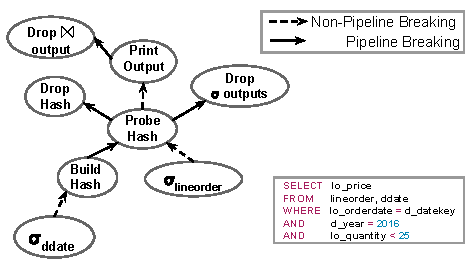
\includegraphics[width=0.9\columnwidth]{figures/QueryPlan}

  \caption{Example of a  query plan produced in Quickstep}~\label{fig:figure1}
  \vspace{-2.0em}
\end{figure}

% BALANCE COLUMNS


% REFERENCES FORMAT
% References must be the same font size as other body text.
\bibliographystyle{SIGCHI-Reference-Format}
\bibliography{sample}

\end{document}

%%% Local Variables:
%%% mode: latex
%%% TeX-master: t
%%% End:
